% TODO: Introduce spoken interaction with tools, agents, embodied systems, and memory.
Full-duplex speech interaction is usually evaluated by whether a system can listen and speak concurrently, manage turn transitions, and respond to interruptions. Once speech models are connected to tools, delegated agents, embodied systems, and persistent memory, however, later speech may need to change more than the current response: it may revise a tool call, transfer task responsibility, redirect a physical action, or invalidate information used in future decisions. We use \textbf{speech-grounded task revisability} to denote the ability to interpret incremental speech as evidence for maintaining, modifying, suspending, or revoking task state, and to propagate that decision consistently through execution, feedback, and memory. TOOL, AGENT, EMB, and MEM identify four scopes of this problem: revising an external operation, assigning control over the revision, changing a physical action, and preserving the revised information over time.

\subsection{Interaction with Tool Environment}
\label{sec:interaction-with-tool-environment}
% TODO: Cover speech-driven tool use and tool orchestration.
Tool interaction forms an information loop between users, agents, and environments. Spoken arguments and constraints emerge incrementally; later corrections may conflict with ongoing operations. Feedback is also delivered progressively, informing subsequent confirmations and revisions. Systems must therefore let new information affect relevant operations and interpret subsequent requests against actual execution and played content.

\paragraph{Intent interpretation and call preparation.}
Forming calls requires distinguishing misrecognized arguments from incomplete requests. Synthetic user-style queries adapt tool embeddings to improve noisy-transcript retrieval~\citep{WEB:isca/zorila26_interspeech}, while Spoken Function Calling conditions output on function schemas and environmental context, marking missing arguments as \texttt{NAN}~\citep{DBLP:journals/corr/abs-2608-05126}. BFCL Audio, Full-Duplex-Bench-v3, and VGBench examine acoustic corruption, disfluency and self-correction, and whether speech addresses the agent, respectively~\citep{WEB:pmlr/v306/mao26b,DBLP:journals/corr/abs-2604-04847,DBLP:journals/corr/abs-2609-32536}. Stream RAG retrieves from speech prefixes, overlapping retrieval with listening~\citep{DBLP:journals/corr/abs-2510-02044}. Heard Enough to Act learns early invocation from supervision marking sufficient tool and argument evidence, but remains limited by false triggers~\citep{WEB:arxiv/2610.34653}. These studies address incomplete or unreliable input, without establishing that the request has stabilized.

\paragraph{Request revision during execution.}
Later speech must be associated with an existing task to affect execution. In simulated streaming-transcript interaction, SIA revises speculative calls through identifiers and dependencies, discarding obsolete returns that have not yet entered context~\citep{DBLP:journals/corr/abs-2605-13360}. Gander routes updates to the active task and, where the backend supports them, handles side questions through read-only forks that preserve the main task's execution context~\citep{DBLP:journals/corr/abs-2609-08977}. StepAudio 3 Realtime distinguishes task updates from unrelated speech; Qwen-Audio-Agent separates task cancellation from speech interruption~\citep{WEB:arxiv/2609.14005,DBLP:journals/corr/abs-2609-25195}. DuplexAgent-RSI records task versions and delivery histories: late returns remain recorded but cannot restore cancelled or superseded work to delivery eligibility~\citep{WEB:arxiv/2610.11299}. This separates execution evidence from permission to deliver results.

\begin{figure}[t]
  \centering
  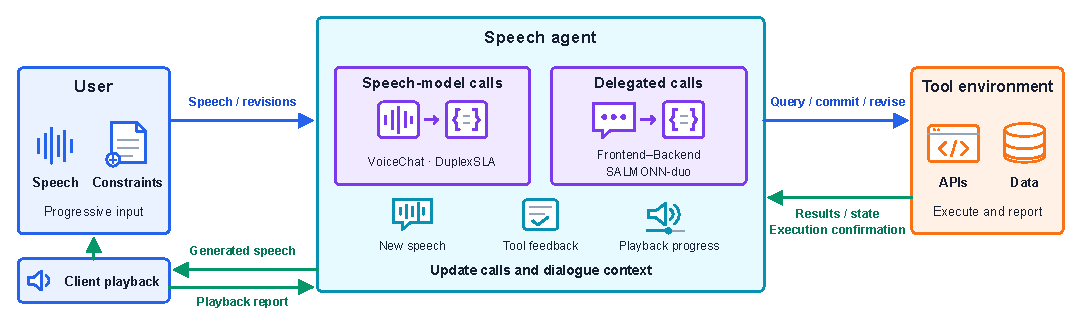
\includegraphics[width=\linewidth]{figures/tool_interaction_loop_en.pdf}
  \caption{The user--agent--environment loop in speech-tool interaction. Blue arrows carry requests and calls; green arrows carry execution feedback, speech delivered through client playback, and playback reports.}
  \label{fig:interaction-with-tools}
\end{figure}

\paragraph{Result integration and spoken feedback.}
Tool completion, integration into generation, and spoken delivery need not coincide. MoshiRAG retrieves between response onset and key content, injecting knowledge into ongoing generation~\citep{DBLP:journals/corr/abs-2604-12928}. GPT-Live distinguishes contextual updates from content to relay aloud; Gemini 3.8 Live's documented non-blocking configuration supports immediate, idle-time, or silent result handling~\citep{WEB:openai/live-delegation,WEB:google/live-capabilities}. Results may become obsolete before a speaking opportunity arises. $\tau$-Voice reports completion claims without corresponding calls~\citep{DBLP:journals/corr/abs-2603-13686}. Qwen-Audio-3.1-Realtime labels pre-call announcements as required, forbidden, or optional~\citep{DBLP:journals/corr/abs-2609-25176}. PACE repairs interrupted dialogue context using playback acknowledgments, avoiding reference to unplayed content~\citep{DBLP:journals/corr/abs-2608-07631}. Interpreting subsequent requests therefore depends on previously delivered information as well as execution state; playback records establish an opportunity to hear, not comprehension.

\paragraph{Call architectures and policy learning.}
Calls can be generated by the speech model or delegated to another decision module. VoiceChat generates structured calls through a separate function channel but excludes execution-time speech from response generation; DuplexSLA aligns speech and actions in shared 160-ms chunks~\citep{DBLP:journals/corr/abs-2609-21967,WEB:arxiv/2605.20755}. Delegated interfaces differ at runtime: Frontend--Backend suppresses frontend output during execution, whereas SALMONN-duo keeps it active and incorporates backend responses based on an invocation-time context snapshot~\citep{DBLP:journals/corr/abs-2609-19334,DBLP:journals/corr/abs-2609-34247}. Qwen3.5-Omni uses text-conditioned responses to supervise audio-conditioned generation~\citep{DBLP:journals/corr/abs-2604-15804}. VoxMind supplies reasoning and tool-use trajectories and retrieves tools on demand; SpeechGym combines call-level feedback with terminal rewards to train tool-use and spoken-response decisions, assuming instantaneous tool execution~\citep{DBLP:conf/acl/LiangCJCJLZPLZ26,DBLP:journals/corr/abs-2608-26432}.

\paragraph{Challenges.}
Speech-tool interaction must balance shorter waits with opportunities for revision. Complete arguments do not imply that the user has finished speaking, and earlier commitment may leave subsequent corrections too late to take effect. Early invocation, task updates, and stale-result filtering address different parts of this process, but revisable task records do not ensure revisable operations. Systems must determine both whether current evidence supports a call and what execution would commit them to, including what later speech could still change.

\paragraph{Outlook.}
Future action policies should adapt to incoming information and execution progress, jointly deciding when to keep listening, clarify, prepare, or commit. Where operations remain revisable, later speech should guide timely execution changes. Where effects have already occurred, systems should identify the limits of revision, explain consequences, and seek feasible remedies. Responsiveness should therefore be considered alongside effective user intervention, so that faster execution does not simply advance an intention that the user has already revised.

\begin{TakeawayBox}{Takeaways: Interaction with Tool Environment}
Speech-tool interaction couples unfolding requests with ongoing operations. Early calls can reduce waiting but may narrow the window for corrections. Returned results and played feedback inform subsequent confirmations and revisions. Systems must adapt actions to new information and execution progress, while distinguishing completed operations from those still changeable, enabling users to refine tasks as work proceeds.
\end{TakeawayBox}

\subsection{Interaction with Agents}
\label{sec:interaction-with-agents}

Full-duplex interaction allows speech to revise a task while an agent is speaking, delegating work, or returning results. Existing systems already use speech for inter-agent messaging, transcript repair, and specialist coordination~\citep{DBLP:journals/corr/abs-2401-03945,DBLP:journals/corr/abs-2601-10223,DBLP:journals/corr/abs-2606-07397}. The remaining issue is not communication alone, but whether responsibility, execution, and feedback stay aligned as the user's intent evolves.

\paragraph{Responsibility across frontend and backend.}
Multi-agent collaboration separates governance, participation, communication, and dialogue-history management~\citep{DBLP:journals/corr/abs-2502-14321,WEB:acl/2025.acl-long.1037}. Voice systems distribute these responsibilities across a responsive frontend, an orchestration layer, and asynchronous workers: Interaction Models and SALMONN-duo retain a conversational frontend, Gander mediates agentic execution through a runtime, and VoxMind and Qwen-Audio-Agent separate dialogue from delegated work~\citep{WEB:thinkingmachines/interaction-models,DBLP:journals/corr/abs-2609-34247,DBLP:journals/corr/abs-2609-08977,DBLP:conf/acl/LiangCJCJLZPLZ26,DBLP:journals/corr/abs-2609-25195}. These components respectively receive evidence, bind it to task state, and execute or verify bounded work.

\paragraph{Decision points within the delegation loop.}
Delegation introduces four decisions: when to launch work, whether later speech supplements or supersedes it, whether execution or only delivery should stop, and whether a returned result remains valid. Existing systems expose complementary controls: Gander reports lifecycle events, Qwen-Audio-Agent separates interruption from cancellation, AdaptDuplex identifies concurrent launches, and Jarvis associates typed decisions with versioned task records~\citep{DBLP:journals/corr/abs-2609-08977,DBLP:journals/corr/abs-2609-25195,DBLP:journals/corr/abs-2609-29217,WEB:arxiv/2610.23804}. A revision is reliable only when the control decision and the affected execution refer to the same task version.

\begin{figure*}[t]
  \centering
  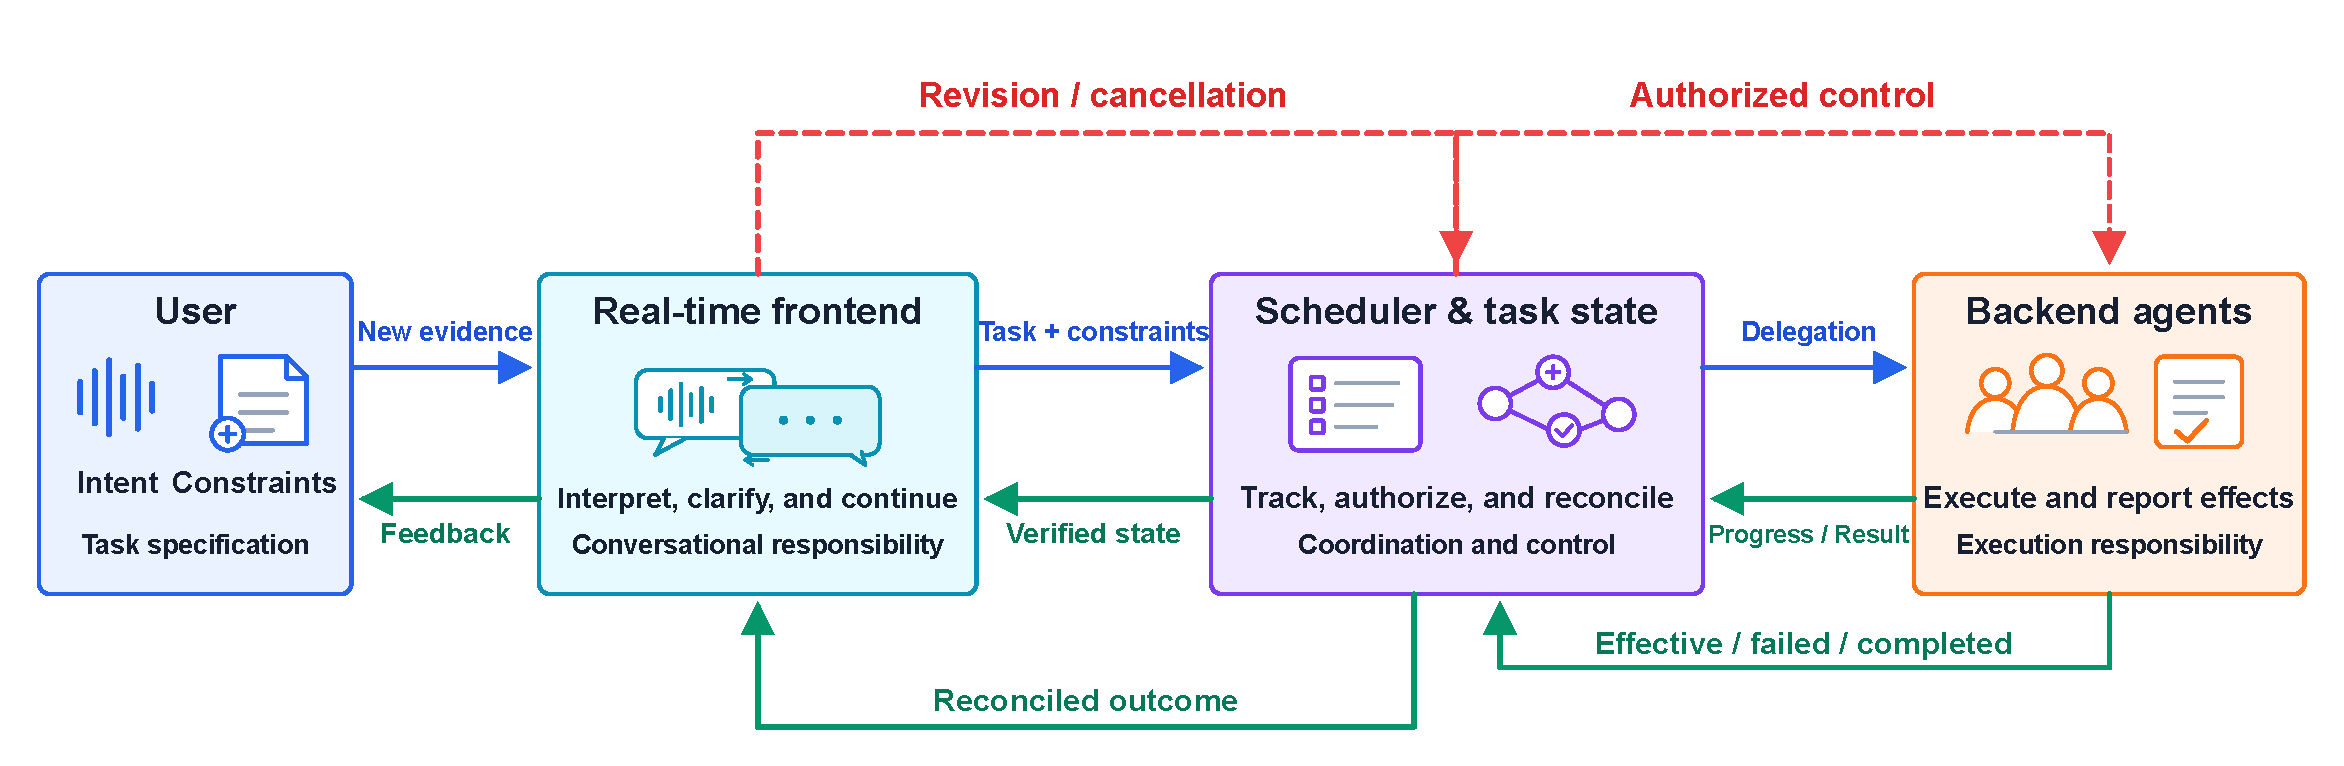
\includegraphics[width=\textwidth]{figures/agents-incremental-feedback.pdf}
  \caption{Information and control loops for a progressively specified task. The real-time frontend maintains the conversation, the scheduler binds new evidence to task state, and backend agents execute bounded work. Blue arrows carry task information, green arrows carry execution evidence, and red dashed arrows carry revision or cancellation.}
  \label{fig:agents-incremental-feedback}
\end{figure*}

\paragraph{Evaluation direction.}
Evaluation should follow revision scenarios rather than count agents or messages. Three measures are central: update latency until a state change is verified, update correctness for accepting the intended version and rejecting stale work, and feedback consistency between execution and what the user hears. Workflow frameworks provide observable state, durable execution, and cancellation primitives~\citep{WEB:google/adk-workflows,WEB:crewai/processes,WEB:microsoft/agent-framework,WEB:langchain/langgraph,WEB:a2a/specification}, while current benchmarks emphasize topology, long-horizon collaboration, protocol, memory, and routing~\citep{DBLP:conf/acl/ZhuDHYGWWQTJY25,DBLP:journals/corr/abs-2609-31590,WEB:arxiv/2610.04672}. Voice evaluation should additionally revise a constraint after delegation, replace a goal in flight, and cancel as a result arrives.

\paragraph{Challenges.}
The primary challenge is version-consistent accountability. Full duplex removes the turn boundary that normally fixes an interpretation before action, so different components may authorize, execute, and report different revisions. Shared context and successful message delivery are insufficient unless stale outcomes are rejected and the system can verify which change actually took effect.

\paragraph{Outlook.}
A promising direction is a speech-aware control layer connecting three accountability surfaces: a frontend that detects new evidence, a scheduler that owns task identity and revision authorization, and a backend that reports execution evidence. Future systems should combine explicit task versions, bounded cancellation, and delivery checks with benchmarks that trace each spoken revision from detection to verified execution and user-visible feedback.

\begin{TakeawayBox}{Takeaways: Interaction with Agents}
Agentic speech interaction requires more than multi-agent communication. Reliable delegation depends on explicit task identity, revision-aware control, stale-result rejection, and feedback grounded in the task version that actually executed.
\end{TakeawayBox}

\subsection{Interaction with Robotic Embodiment}
\label{sec:interaction-with-robotic-embodiment}
Speech enables users to specify and revise embodied tasks as execution changes the environment. Effective interaction links spoken intent to physical control and uses observed outcomes to guide subsequent planning and dialogue. Figure~\ref{fig:embodied-speech-overview} summarizes this revisable process.

\begin{figure}[!htbp]
  \centering
  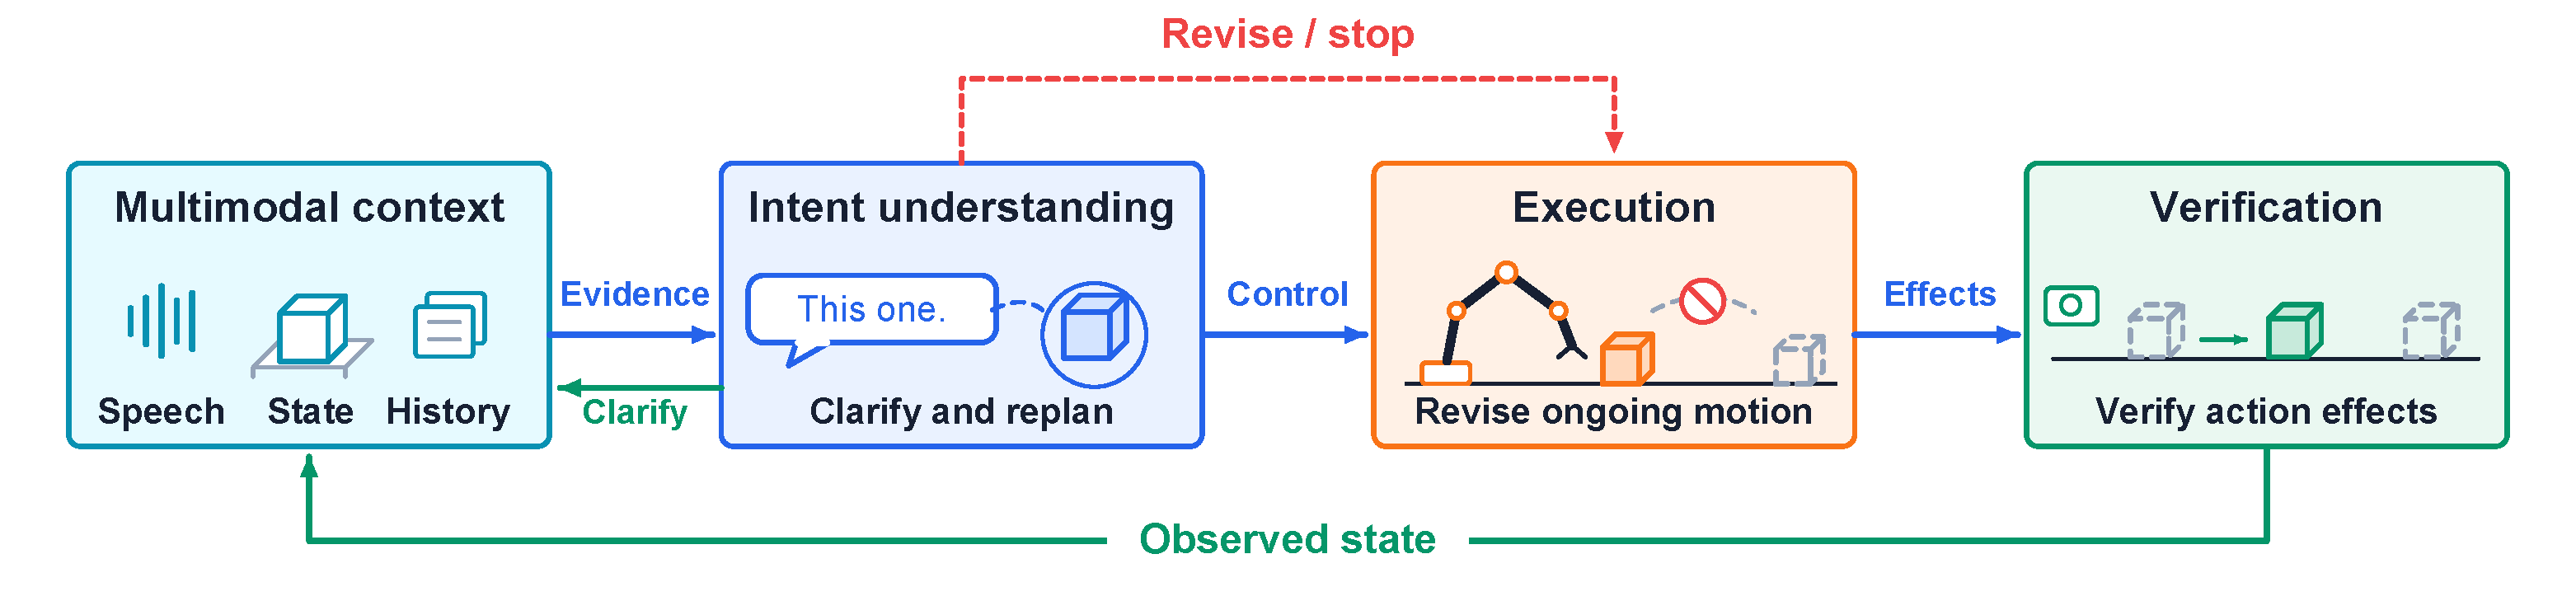
\includegraphics[width=\linewidth]{figures/embodied_speech_overview.pdf}
  \caption[Embodied speech interaction loop]{Embodied speech interaction as a revisable physical loop. Speech, current state, and interaction history inform intent understanding and planning. Blue arrows carry evidence, control, and action effects; the red dashed path denotes revision or stopping, and green arrows return clarification and observed state. Dashed object outlines represent prior or unexecuted positions. Full-duplex speech supports concurrent listening and speaking. Effective physical revision requires controller responses within temporal and safety limits, with subsequent planning and spoken feedback based on the state actually reached.}
  \label{fig:embodied-speech-overview}
\end{figure}

\paragraph{Intent Understanding and Clarification.}
Understanding spoken intent requires integrating speech with the current scene and task context. Visual context improves recognition of synthetically corrupted instructions~\citep{emb_chang2023}, while modular ASR--language--vision integration supports robot command generation~\citep{emb_nwankwo2024}. NMM-HRI combines pointing and RGB-D observations for reference resolution; VLAS conditions manipulation on speech and images and retrieves speaker-specific knowledge~\citep{emb_lai2025nmm,emb_zhao2025vlas}. When intent remains uncertain, dialogue can clarify the task before execution. RoboOmni infers intent from conversation, environmental sounds, and vision, then requests spoken confirmation before manipulation~\citep{emb_wang2025roboomni}. KnowNo complements these approaches by addressing when language-based robot planners should seek human assistance~\citep{emb_ren2023knowno}.

\paragraph{Revision, Replanning, and Feedback.}
Once execution begins, users can revise goals or constraints in response to observed behavior. Interactive Language accepts successive spoken instructions via ASR~\citep{emb_lynch2022interactive}; YAY Robot accepts a verbal stop followed by correction and incorporates interventions into subsequent policy learning~\citep{emb_shi2024yay}. Incremental language understanding coupled with online motion planning allows trajectories and constraints to change as an instruction unfolds~\citep{emb_abrams2025incremental}. Since revision does not erase prior physical effects, replanning must combine the updated instruction with the observed robot and scene state. HEAR preserves transient acoustic evidence across execution gaps for later control decisions~\citep{emb_nie2026hear}. Spoken feedback should convey observed progress, deviations, and uncertainty, giving users a basis for further correction or confirmation.

\paragraph{Full-Duplex Interaction.}
Full-duplex systems support intervention during robot speech through concurrent listening and speaking, incorporating incoming speech into the ongoing interaction. ELLSA coordinates modalities within a streaming model and evaluates action barge-in in simulation~\citep{emb_wang2026ellsa}; VITA-E uses parallel active and standby models for concurrent interaction, task switching, and stop requests on a physical humanoid~\citep{emb_liu2025vitae}. MIRA combines speech interruption handling with short, cancellable motion prefixes in companion interaction~\citep{emb_lin2026mira}. Deployment constraints remain relevant: the Pepper framework mutes its microphone during speech output because it lacks echo cancellation~\citep{emb_studerus2026pepper}. Beyond speech reception, physical responsiveness depends on how interventions reach and update the controller.

\paragraph{Challenges.}
Concurrent interaction must accommodate the different timescales of speech and physical execution. Recognition errors can redirect actions, while incomplete utterances, self-repairs, and overlapping speech make early interpretations provisional. Causal streaming restricts decisions to available evidence; buffering and committed motion can delay correction until physical effects are irreversible. VAP addresses conversational turn prediction, and RASSG studies repair-aware cancellation under simulated tool execution~\citep{emb_inoue2024vap,emb_hu2026rassg}. Applying these mechanisms to robots requires validation across speech reception, controller updates, physical stopping, and task outcomes. Evaluation must also establish whether replanning and spoken reports remain consistent with the resulting state.

\paragraph{Outlook.}
In future long-horizon assistance and collaborative manipulation, speech could serve as an incremental task specification. Users could start with an approximate goal and refine preferences, references, and constraints while observing execution. By integrating these updates with interaction history and current observations, robots could maintain a revisable interpretation of intent, adapt their plans, and seek clarification before committing to uncertain actions. Spoken output would make this process accessible by distinguishing completed steps, current progress, unresolved uncertainty, and intended next actions. Such exchanges could support the continuous joint refinement of tasks, bringing robot behavior into closer alignment with users' evolving goals.

\begin{TakeawayBox}{Takeaways: Interaction with Robotic Embodiment}
Speech supports incremental task refinement; full-duplex interaction permits intervention during system speech. Effective revision requires control updates within task-specific temporal and safety limits, followed by replanning from observed physical outcomes. Accurate spoken feedback enables further correction and confirmation, sustaining alignment with evolving user goals.
\end{TakeawayBox}




\subsection{Interaction with Self-Memory and Lifelong Context}
\label{sec:interaction-with-memory}

Memory enables spoken dialogue systems to maintain information beyond the current utterance and reuse it across later interactions. In full-duplex dialogue, however, interpretations may change as speech unfolds, making it necessary to distinguish provisional evidence from confirmed information and preserve the validity of subsequent revisions. Effective memory interaction therefore concerns not only what is retained, but when information becomes valid and whether superseded information continues to influence later decisions. Figure~\ref{fig:memory-overview} illustrates this process.

\begin{figure}[!htbp]
\centering
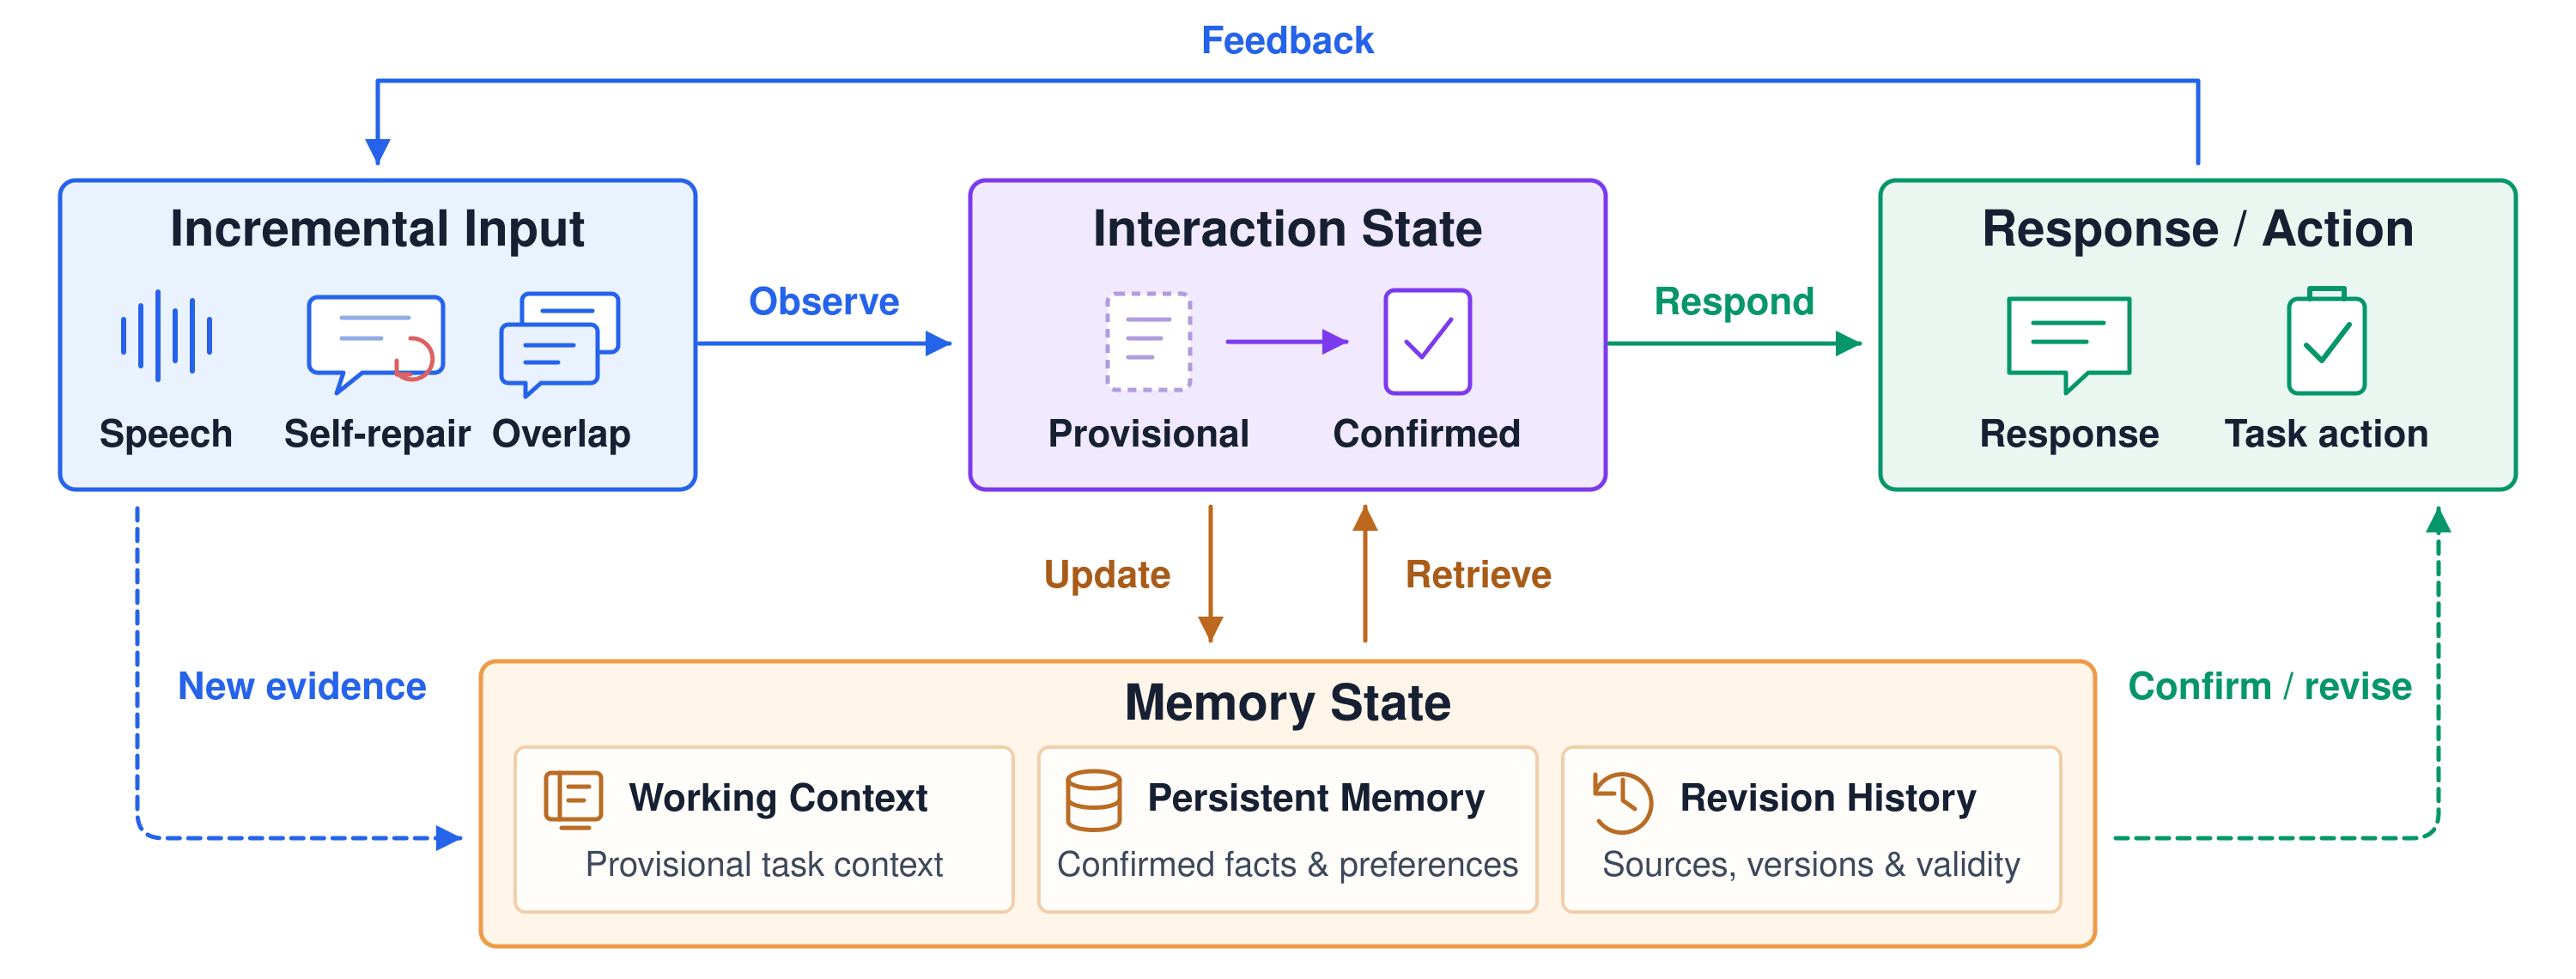
\includegraphics[width=\linewidth]{figures/memory_overview.png}
\caption{Memory-supported interaction in full-duplex spoken dialogue. Incremental speech and interaction context inform memory formation, retrieval, revision, and persistence. Corrections and deletions may change the validity of stored information and its use in subsequent interactions.}
\label{fig:memory-overview}
\end{figure}

\paragraph{Memory Formation and Attribution.}
Forming persistent memory requires selecting information from ongoing interaction and preserving its source and conversational context. EgoMem processes audiovisual streams through asynchronous retrieval, dialogue, and memory management, using detected interaction boundaries to extract and update user information~\citep{DBLP:journals/corr/abs-2509-11914}. In multi-party settings, attribution becomes more complex. VoiceTrace supports speaker-conditioned speech retrieval~\citep{DBLP:journals/corr/abs-2609-18521}, while SpeakerMem-R1 organizes speaker-labeled messages and derived personal and group states~\citep{DBLP:journals/corr/abs-2609-26780}. VoxPolyMem further represents participant relationships and interaction history to support memory retrieval across multi-party spoken sessions~\citep{DBLP:journals/corr/abs-2609-32522}. Beyond lexical content, VoiceMem distinguishes context-dependent affective evidence from more persistent user characteristics~\citep{DBLP:journals/corr/abs-2608-26005}. These approaches improve memory construction and attribution, but identifying the speaker or extracting a fact does not establish whether an incomplete, inferred, or corrected statement should become persistent memory. In full-duplex interaction, such commitment must account for subsequent clarification and self-repair.

\paragraph{Temporal Revision and Memory Updating.}
Persistent information may change across turns and sessions, requiring memory systems to distinguish current facts from their historical versions. Zep represents evolving information through a temporal knowledge graph, preserving source-linked episodes and the validity of relationships~\citep{DBLP:journals/corr/abs-2501-13956}. BELIEFMEM treats conversational updates as belief revisions, maintaining predecessor relationships between superseded and current beliefs~\citep{meng-etal-2026-beliefmem}. APEX-MEM retains temporal history in an append-only property graph and resolves conflicting information during retrieval~\citep{DBLP:conf/acl/BanerjeeMSMC26}, while TSHMem incorporates temporal constraints into graph-based evidence selection to reduce retrieval of outdated information~\citep{xu-etal-2026-tshmem}. For spoken interaction, VoiceMem performs asynchronous memory reconciliation through add, update, delete, and keep operations~\citep{DBLP:journals/corr/abs-2608-26005}. Voice Memory for Agentic Speech Recognition similarly uses an editable memory file and score-gated updates to constrain recognition correction without parameter changes~\citep{DBLP:journals/corr/abs-2607-26410}. These mechanisms address different parts of memory revision. However, updating a stored record or selecting the correct version at retrieval does not necessarily invalidate information already incorporated into summaries, user profiles, cached context, or ongoing tasks.

\paragraph{Persistent Memory and Evaluation.}
Reliable memory revision must remain effective beyond the turn in which a correction occurs. LongMemEval evaluates knowledge updates and temporal reasoning across extended conversational histories~\citep{DBLP:conf/iclr/WuWYZCY25}, while ChronoScope examines whether temporal scope is preserved or revised across successive dialogue turns~\citep{DBLP:conf/acl/AtriJH26}. For spoken interaction, VoxMem evaluates multi-session memory involving speech content, speaker identity, paralinguistic information, and temporal tracking~\citep{DBLP:journals/corr/abs-2609-32607}. ContextDialog examines conversational context recall and utilization in voice interaction models~\citep{contextdialog}. Beyond answer correctness, MemEval diagnoses failures across memory extraction, updating, retrieval, and utilization~\citep{wang-etal-2026-memories}, and UTILMEM examines whether retrieved evidence is integrated reliably into downstream responses~\citep{qing-etal-2026-utilmem}. Together, these evaluations expose limitations in temporal reasoning, attribution, and memory utilization. Yet correctly answering a question about a revised fact does not by itself establish that obsolete information has been invalidated throughout persistent storage or excluded from subsequent task decisions.

\paragraph{Challenges.}
Memory revision in full-duplex dialogue faces both temporal and state-consistency constraints. Incomplete utterances, overlapping speech, and self-repairs make it difficult to determine when information should be committed, while speaker identification alone cannot establish addressee, conversational function, or authority to modify a record. Once committed, corrections must propagate beyond the original memory entry. Forgetting Without Restarting demonstrates that deleting explicit memory can leave revoked information influential through derived execution state, and investigates provenance-guided replay to address this problem~\citep{DBLP:journals/corr/abs-2609-04875}. Comparable consistency requirements arise across summaries, retrieval indexes, speaker profiles, and pending task operations. Deletion must also be distinguished from historical invalidation, and task cancellation from factual correction. Current evaluations rarely inspect these states together under continuous speech. Establishing reliable revision therefore requires measuring when an update takes effect, which representations remain affected, and whether outdated evidence still changes subsequent behavior.

\paragraph{Outlook.}
Future spoken agents could maintain versioned, source-aware memory in which provisional interpretations, confirmed facts, historical records, and deleted information have explicitly distinguished roles. Incremental speech processing would support early retrieval and response preparation without prematurely committing uncertain evidence. Corrections could then update the active memory state, preserve appropriate historical relationships, and trigger revalidation of dependent summaries, retrievals, and tasks. For multi-party interaction, such mechanisms would additionally track speaker attribution, participation, and conversational authority. Evaluation should follow a revision from its initial utterance through confirmation, storage, retrieval, and subsequent decisions, including across sessions. This would shift lifelong memory assessment from recalling prior conversations toward verifying that evolving information remains consistent with the system's ongoing behavior.

\begin{TakeawayBox}{Takeaways: Self-Memory and Lifelong Context}
Memory-level revisability requires distinguishing provisional speech interpretations from committed information, preserving source and temporal validity, and preventing superseded records from influencing current decisions. Existing work advances memory attribution, temporal updating, and cross-session evaluation, but reliable propagation across stored representations and ongoing task state remains insufficiently established.
\end{TakeawayBox}

